\documentclass[../../main.tex]{subfiles}
\graphicspath{{../../image/}{../../figure/}}
\begin{document}

\section{K均值聚类}\label{section:ch15-k均值}

我们首先考虑在多维空间中识别数据点群组或聚类的问题。假设有一个数据集 $\{\bm{x}_1,\cdots,\bm{x}_N\}$，其中包含了 $N$ 个 $D$ 维欧几里得变量 $\bm{x}$ 的观测值。我们的目标是将该数据集划分成 $K$ 个聚类，可以暂定 $K$ 的值是已知的。直觉上，我们会认为一个聚类包含一组数据点，这些数据点之间的距离相较于聚类外的数据点之间的距离要短。这里引入一组 $D$ 维向量 $\bm{\mu}_k$，其中 $k=1,\cdots,K$，并且 $\bm{\mu}_k$ 是第 $k$ 个聚类的“原型”。可以认为 $\bm{\mu}_k$ 代表了聚类中心。然后要找到一组聚类向量 $\{\bm{\mu}_k\}$，以及数据点到聚类的分配，使得每个数据点到与其最近的聚类向量 $\bm{\mu}_k$ 的距离平方和最小。

为了方便起见，需要定义一些符号来描述数据点到聚类的分配。对于每个数据点 $\bm{x}_n$，我们引入相应的一组二进制指示变量 $r_{nk}\in\{0,1\}$，其中 $k=1,\cdots,K$。这些指示变量描述了数据点 $\bm{x}_n$ 会被分配到哪个聚类，因此如果数据点 $\bm{x}_n$ 被分配到聚类 $k$，那么 $r_{nk}=1$，并且对于 $j\neq k$，$r_{nj}=0$。这是~1-of-$K$~编码方案的一个例子。接下来可以定义如下误差函数：
\begin{align}
J=\sum_{n=1}^{N}\sum_{k=1}^{K}r_{nk}\,\|\bm{x}_n-\bm{\mu}_k\|^2
\label{align:ch15-kmeans-loss}
\end{align}
该误差函数代表每个数据点到分配给它的聚类向量 $\bm{\mu}_k$ 的距离平方和。我们的目标是找到 $\{r_{nk}\}$ 和 $\{\bm{\mu}_k\}$ 的值，让 $J$ 最小。这可以通过一个迭代过程来实现，其中每次迭代包括两个连续步骤，分别对应于对 $\{r_{nk}\}$ 和 $\{\bm{\mu}_k\}$ 进行的连续优化。首先为 $\{\bm{\mu}_k\}$ 选择一些初始值。然后在第一步，保持 $\{\bm{\mu}_k\}$ 固定，并优化 $\{r_{nk}\}$ 以最小化 $J$；而在第二步，保持 $\{r_{nk}\}$ 固定，并优化 $\{\bm{\mu}_k\}$ 以最小化 $J$。重复这两步优化直至收敛。

在第一步，保持 $\{\bm{\mu}_k\}$ 固定，并关于 $\{r_{nk}\}$ 最小化 $J$。$J$ 是关于 $\{r_{nk}\}$ 的线性函数，所以对于这个优化可以轻松地给出闭合形式的解。涉及不同 $n$ 的项是独立的，因此对于任何能给出 $\|\bm{x}_n-\bm{\mu}_k\|^2$ 最小值的 $k$ 值，可以通过选择 $r_{nk}=1$ 来单独为每个 $n$ 进行优化。换句话说，我们只是简单地将第 $n$ 个数据点分配给与其最近的聚类，这可以表示为
\begin{align}
r_{nk}=
\begin{cases}
1, & k=\arg\min_j\|\bm{x}_n-\bm{\mu}_j\|^2\\
0, & \text{其他}
\end{cases}
\label{align:ch15-kmeans-assign}
\end{align}

接下来考虑在 $\{r_{nk}\}$ 固定的情况下优化 $\{\bm{\mu}_k\}$（M~步骤）。目标函数 $J$ 是关于 $\bm{\mu}_k$ 的二次函数，可通过将其关于 $\bm{\mu}_k$ 的导数设为零来最小化它，从而得到
\begin{align}
\sum_{n=1}^{N}r_{nk}(\bm{x}_n-\bm{\mu}_k)=0
\label{align:ch15-kmeans-mu-deriv}
\end{align}
我们可以很容易地解出 $\bm{\mu}_k$，得到
\begin{align}
\bm{\mu}_k=\frac{\sum_n r_{nk}\bm{x}_n}{\sum_n r_{nk}}.
\label{align:ch15-kmeans-mu}
\end{align}

观察式\eqref{align:ch15-kmeans-mu}的右侧，分母等于分配给聚类 $k$ 的数据点的数量，运算结果 $\bm{\mu}_k$ 可以简单地看作等于所有分配给聚类 $k$ 的数据点 $\bm{x}_n$ 的平均值。这种方法因而得名~K~均值算法（Lloyd, 1982）。因为 $\{r_{nk}\}$ 是离散的，并且每次迭代都不会导致误差函数增大，所以~K~均值算法一定可以在有限的步骤中收敛（见习题~15.1）。

\begin{figure}[htbp]
\centering
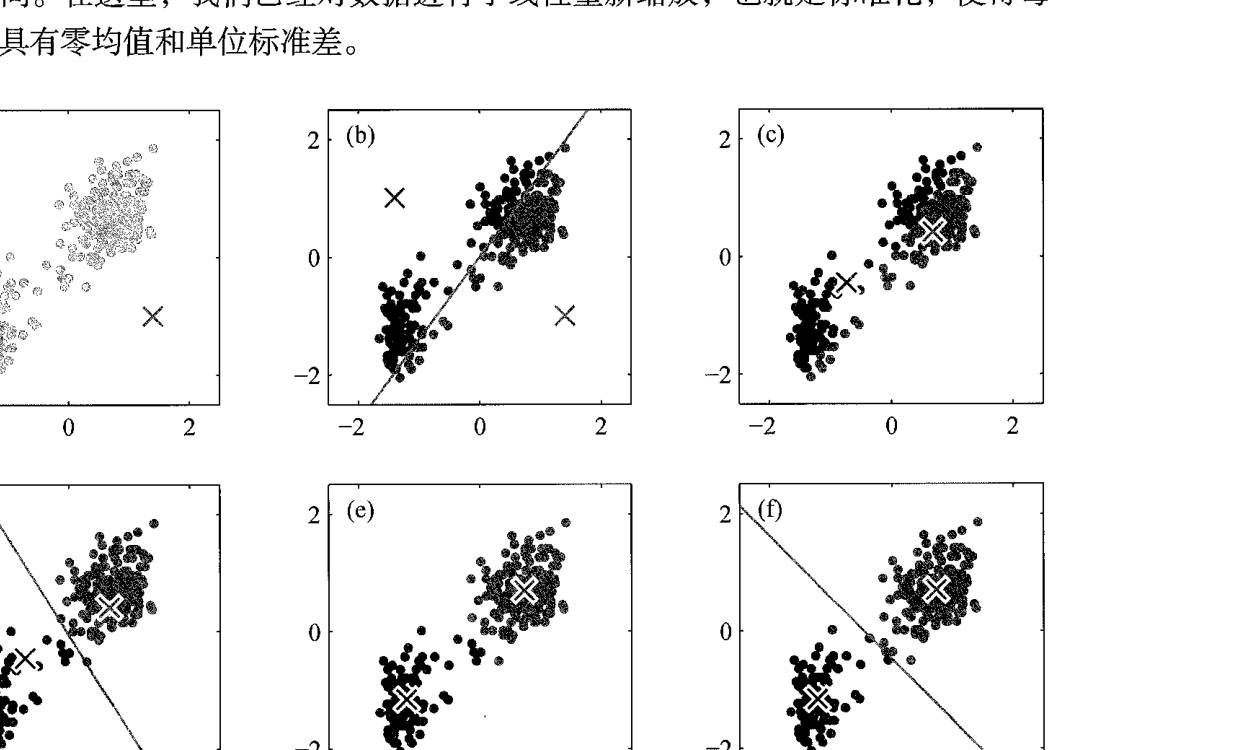
\includegraphics[width=0.9\textwidth]{ch15-fig15.1-kmeans.png}
\caption{利用线性重新缩放的老忠实喷泉数据集来说明~K~均值算法。(a)~绿色点代表二维欧几里得空间中的数据集，红色和蓝色的叉号表示初始选择的聚类中心；(b)~在初始的~E~步骤中，每个数据点要么分配给红色聚类，要么分配给蓝色聚类；(c)~在随后的~M~步骤中，每个聚类中心被重新计算为分配给对应聚类的所有数据点的平均值；(d)--(i)~显示了直至最终收敛前的连续~E~步骤和~M~步骤。}
\label{fig:ch15-kmeans}
\end{figure}

将数据点重新分配到聚类和重新计算聚类均值这两个阶段轮流重复进行，直至分配不再变化（或者直至迭代次数超过某预定值）。然而，这种方法可能会收敛到目标函数 $J$ 的局部极小值而不是全局最小值。MacQueen (1967) 研究了~K~均值算法的收敛性。

\cref{fig:ch15-kmeans}使用源自美国黄石国家公园老忠实喷泉（Old Faithful geyser）数据集的喷发数据对~K~均值算法进行了说明（参见~3.2.9~小节）。该数据集包含~272~个数据点，每个数据点都在水平轴上给出了一次喷发的持续时间，并在垂直轴上给出了下一次喷发的持续时间。在这里，我们已经对数据进行了线性重新缩放，也就是标准化，使得每个变量都具有零均值和单位标准差。

到目前为止，考虑的是批量版本的~K~均值算法，其中整个数据集一起用来更新原型向量。我们也可以推导出一个顺序更新的策略，在这个策略中，对于每个数据点 $\bm{x}_n$，更新离它最近的原型向量 $\bm{\mu}_k$：
\begin{align}
\bm{\mu}_k^{\text{new}}=\bm{\mu}_k^{\text{old}}+\frac{1}{N_k}(\bm{x}_n-\bm{\mu}_k^{\text{old}})
\label{align:ch15-kmeans-online}
\end{align}
其中 $N_k$ 是到目前为止用来更新 $\bm{\mu}_k$ 的数据点的数量。这允许每个数据点在使用一次后就被丢弃，然后处理下一个数据点。

K~均值算法的一个显著特点是，在每次迭代中，每个数据点都只被分配给一个聚类。尽管有些数据点会比其他任何聚类中心 $\bm{\mu}_j$ 更接近特定聚类中心 $\bm{\mu}_k$，但也可能有其他数据点大约处于聚类中心之间的中点位置。在后一种情况下，其实并不清楚将数据点硬性分配给最近的聚类是否是最合适的方法。我们将看到，通过采用概率方法，我们将能够以一种反映最适当分配的不确定性程度的方式，获得数据点到聚类的“软”分配。这种概率方法有许多好处。

作为~K~均值算法应用的例子，我们考虑图像分割和图像压缩这两个相关问题。图像分割的目标是将图像划分成区域，以便每个区域都具有相对一致的视觉外观或者对应于物体或物体的某一部分（Forsyth and Ponce, 2003）。图像中的每个像素都是由红、绿、蓝通道的强度组成的三维空间中的一个点，图像分割算法简单地将图像中的每个像素作为一个单独的数据点来处理。然后展示了对任何特定的 $K$ 值运行~K~均值算法直至收敛的结果，方法是重新绘制图像，并替换图像中的每个像素向量——用其分配到的聚类中心 $\bm{\mu}_k$ 给出的 $\{R,G,B\}$ 强度三元组进行替换。各种不同 $K$ 值的结果表明，对于给定的 $K$ 值，该算法只使用 $K$ 种颜色来表示图像。

我们也可以使用聚类算法进行数据压缩。首先我们要区分无损数据压缩（其目标是从压缩表示中精确地重建原始数据）和有损数据压缩（也就是说，我们接受数据重建过程中的一些误差以换取相比无损压缩情况下更高的压缩率）。我们可以将~K~均值算法应用于有损数据压缩问题。对于 $N$ 个数据点中的每一个数据点，我们只存储其分配到的聚类的身份 $k$。我们还需要存储 $K$ 个聚类中心 $\{\bm{\mu}_k\}$ 的值，在我们选择 $K\ll N$ 的前提下，这种方法明显减少了需要的数据量，然后每个数据点都可以通过与其最近的聚类中心 $\bm{\mu}_k$ 来近似表示。新的数据点同样可以通过首先找到最近的 $\bm{\mu}_k$，然后存储标签 $k$ 而不是原始的数据向量来进行压缩。这个框架通常称为向量量化（vector quantization），向量 $\{\bm{\mu}_k\}$ 称为码本向量（codebook vector）。

\end{document}
